\documentclass[10pt, french]{article}
\usepackage[landscape, hmargin=1cm, vmargin=1.7cm]{geometry}
\usepackage{tikz}
\usepackage{csquotes}

%% -----------------------------
%% Préambule
%% -----------------------------
% !TEX encoding = UTF-8 Unicode
% LaTeX Preamble for all cheatsheets
% Author : Gabriel Crépeault-Cauchon

% HOW-TO : copy-paste this file in the same directory as your .tex file, and add in your preamble the next command right after you have specified your documentclass : 
% \input{preamble-cheatsht.tex}
% ---------------------------------------------
% ---------------------------------------------

% Extra note : this preamble creates document that are meant to be used inside the multicols environment. See the documentation on internet for further information.

%% -----------------------------
%% Encoding packages
%% -----------------------------

%% -----------------------------
%% Fontawesome for special symbols
%% -----------------------------
\usepackage{fontspec}
%\defaultfontfeatures{Path = /usr/local/texlive/⁨2018⁩/texmf-dist⁩/fonts/opentype/public/fontawesome/}
\defaultfontfeatures{Extension = .otf}
\usepackage{fontawesome}
\usepackage[utf8]{inputenc}
\usepackage[T1]{fontenc}
\usepackage{babel}
\usepackage{lmodern}
\usepackage[colorinlistoftodos]{todonotes}
%% -----------------------------
%% Variable definition
%% -----------------------------
\def\auteur{\href{https://github.com/ressources-act/Guide_de_survie_en_actuariat/blob/master/02_Cheatsheets/contributeurs/contributeurs-cheatshts.pdf}{\faGithub \ Liste des contributeurs}}
\def\BackgroundColor{white}
\usepackage{xargs} % for more logical new function creation

%% -----------------------------
%% Margin and layout
%% -----------------------------
% Determine the margin for cheatsheet
\usepackage[landscape, hmargin=1cm, vmargin=1.7cm]{geometry}
\usepackage{multicol}
\usepackage{multirow}

% Remove automatic indentation after section/subsection title.
\setlength{\parindent}{0cm}

% Save space in cheatsheet by removing space between align environment and normal text.
\usepackage{etoolbox}
\newcommand{\zerodisplayskips}{%
  \setlength{\abovedisplayskip}{0pt}%
  \setlength{\belowdisplayskip}{0pt}%
  \setlength{\abovedisplayshortskip}{0pt}%
  \setlength{\belowdisplayshortskip}{0pt}}
\appto{\normalsize}{\zerodisplayskips}
\appto{\small}{\zerodisplayskips}
\appto{\footnotesize}{\zerodisplayskips}

%% -----------------------------
%% URL and links
%% -----------------------------
\usepackage{hyperref}
\hypersetup{colorlinks = true, urlcolor = gray!70!white, linkcolor = black}

%% -----------------------------
%% Document policy (uncomment only one)
%% -----------------------------
%	\usepackage{concrete}
	\usepackage{mathpazo}
%	\usepackage{frcursive} %% permet d'écrire en lettres attachées
%	\usepackage{aeguill}
%	\usepackage{mathptmx}
%	\usepackage{fourier} 

%% -----------------------------
%% Math configuration
%% -----------------------------
\usepackage{ctable} % for \specialrule command
\usepackage[fleqn]{amsmath}
\usepackage{amsthm,amssymb,latexsym,amsfonts}
\usepackage{textcomp} %% j'avais un avertissement, voir https://latex.org/forum/viewtopic.php?f=4&t=3364#p13124 pour pourquoi j'import ce paquetage
\usepackage{gensymb}
\usepackage{empheq}
\usepackage{numprint}
\usepackage{dsfont} % Pour avoir le symbole du domaine Z
%\usepackage{bigints} % pour des gros intégrales
% Mathematics shortcuts
\usepackage{scalerel,stackengine,amsmath}
\newcommand\equalhat{\mathrel{\stackon[1.5pt]{=}{\stretchto{%
    \scalerel*[\widthof{=}]{\wedge}{\rule{1ex}{3ex}}}{0.5ex}}}}
%%	Créé des cercles avec des chiffres
%%	Example usage:	\circled{1} [creates an inline circle with 1]
%%		+	Within a list, \begin{enumerate}[label = \circled{\arabic*}]
\DeclareRobustCommand*\circled[2]{%
	\tikz[baseline = (char.base)]{%
		\node[%
			shape = circle,%
			fill = #2!40,%	inner circle
			draw = #2,%		outer rim
			inner sep = 2pt%
		] (char) {#1};%
	}%
} 
\DeclareRobustCommand*\ellipsed[2]{%
	\tikz[baseline = (char.base)]{%
		\node[%
			shape = rectangle,%
			fill = #2!40,%	inner circle
			draw = #2,%		outer rim
			inner sep = 2pt,%
			rounded corners = 4pt
		] (char) {#1};%
	}%
} 
\DeclareRobustCommand*\rectangled[2]{%
	\tikz[baseline = (char.base)]{%
		\node[%
			shape = rectangle,%
			fill = #2!40,%	inner circle
			draw = #2,%		outer rim
			inner sep = 2pt%
		] (char) {#1};%
	}%
} 
\newcommand{\reels}{\mathbb{R}}
\newcommand{\entiers}{\mathbb{Z}}
\newcommand{\naturels}{\mathbb{N}}
\newcommand{\eval}{\biggr \rvert}
\usepackage{cancel}
\newcommand{\derivee}[1]{\frac{\partial}{\partial #1}}
\newcommand{\prob}[1]{\Pr \left( #1 \right)}
\newcommand{\esp}[1]{\mathrm{E} \left[ #1 \right]} % espérance
\newcommand{\variance}[1]{\mathrm{Var} \left( #1   \right)}
\newcommand{\covar}[1]{\mathrm{Cov} \left( #1   \right)}
\newcommand{\laplace}{\mathcal{L}}
\newcommand{\deriv}[3][]{\frac{\partial^{#1}#3}{\partial #2^{#1}}}
\newcommand{\e}[1]{\mathrm{e}^{#1}}
\newcommand{\te}[1]{\text{exp}\left\{#1\right\}}
\DeclareMathSymbol{\shortminus}{\mathbin}{AMSa}{"39}
%%	Example usage:	\sumz{n}{i = 1} <=> \overset{n}{\underset{i = 1}{\sum}}
\newcommand{\sumz}[2]{\overset{#1}{\underset{#2}{\sum}}}
%%	Example usage:	\limz{h}{0} <=> \underset{h \rightarrow 0}{\lim}
\newcommand{\limz}[2]{\underset{#1 \rightarrow #2}{\lim}}
%%	Example usage:	\LVx{h}	<=>	\actsymb[h]{L}{}[]
%%					\LVx[n]{h}	<=>	\actsymb[h]{L}{}[n]
\newcommand{\LVx}[2][]{\actsymb[#2]{L}{}[#1]}
\DeclareMathOperator*{\argmax}{arg\,max}
\DeclareMathOperator*{\argmin}{arg\,min}
%%%	\icbox{<frame color>}{<background color>}{<text>}
\newcommandx{\icbox}[3][1 = bleudefrance, 2 = beaublue]{\fcolorbox{#1}{#2}{#3}}
%%	other good color combo is azure(colorwheel) arsenic
\usepackage{longfbox}
%	voir cette page, paquetage avec CSS https://ctan.math.illinois.edu/macros/latex/contrib/longfbox/longfbox.html
\newfboxstyle{rappel}{
	background-color = tealblue!20!white, 
	border-style = outset,
	breakable = true,
%	
	border-color = tealblue,
	border-radius = 1ex, 
%
	padding-bottom = 0.2ex,
	padding-top = 0.2ex,
	padding-left = 0.4ex,
	padding-right = 0.4ex,
%	
	border-top-width = 0.3ex,
	border-bottom-width = 0.3ex,
%
	border-left-width = 1ex, 
	border-bottom-left-radius = 0.2ex,
%	
	border-right-width = 1ex, 
	border-top-right-radius = 0.2ex,
%	
}
\newfboxstyle{formula}{ 
	background-color = beaublue, 
	border-color = bleudefrance
}
\newfboxstyle{imphl}{ 
	padding = 0pt,
	margin = 0pt,
	baseline-skip = false,
	background-color = palechestnut!60!white, 
	border-color = white
}
\newfboxstyle{conditions}{ 
	background-color = palechestnut, 
	border-color = red
}
\newcommandx{\rcbox}[3][1 = bleudefrance, 2 = beaublue]{\lfbox[border-radius = 0.5ex, background-color = #2, border-color = #1]{#3}}

% To indicate equation number on a specific line in align environment
\newcommand\numberthis{\addtocounter{equation}{1}\tag{\theequation}}

%
% Actuarial notation packages
%
\usepackage{actuarialsymbol}
\usepackage{actuarialangle}

%
% Matrix notation for math symbols (\bm{•})
%
\usepackage{bm}
% Matrix notation variable (bold style)
\newcommand{\matr}[1]{\mathbf{#1}}



%% -----------------------------
%% tcolorbox configuration
%% -----------------------------
\usepackage[many]{tcolorbox}
\tcbuselibrary{xparse}
\tcbuselibrary{breakable}
%%%	Explanation of various arugments : 
%%	colframe:	colour of the rim.
%%	ex.:	colframe	=	blue
%%	colback:		colour of the box.
%%	ex.:	colback	=	blue
%%	--------
%%	fonttitle: 	font of the title
%%	ex.:	fonttitle	=	\bfseries
%%	title: 	actual title text.
%	ex.:	title	=	Reasons why LaTeX is useful
%%	--------
%%	arc:			arc of corners' turn.
%%	ex.:	arc	=	12pt
%%	+	an arc of 0 implies a rectangle.
%%	< type > corners = < location >: 	Creates < type > corners at the specified location.
%	ex.:	 sharp corners	(creates sharp corners for all corners)
%	ex.:	 rounded corners = north (creates round corners for top 2 corners)
%%	+	See pages 34 to 35 for a visualisation of the different types and locations.
%%	+	We can specify rounded corners after a sharp corners to obtain sharp corners everywhere but one place.
%%	--------
%%	attach boxed title to < where > = {}: 	Creates a seperate box for the title.
%%	ex.:	attach boxed title to top center
%%	+	Arguments in parantheses are optional and be used to shift the position.
%%	ex.:	yshift	=	-\tcboxedtitleheight/2
%%	ex.:	xshift	=	2mm
%%	boxed title style = {}: 	Modifies style of box which has same functions as a regular tcb.
%%	<where>rule:		Modifies width of border.
%	ex.:	bottomrule = 2mm
%%	frame style tile={width=1cm}{pink_marble.png} can set a background image for the title box
%%	

%%
%% 	Generalized colour box for definitions
%%
%%	Example usage: \begin{definitionGENERAL}{< title >}[< symbol before title >][< color >]
\DeclareTColorBox{definitionGENERAL}{
	m 
	o
	O{amber(sae/ece)}
}
{
	enhanced,
	colback			=	#3!5!white, 
	arc				=	12pt,
	sharp corners,
%	watermark tikz	=	{
%		\draw[line width = 2mm] circle (1cm) node{
%			\fontfamily{ptm}
%			\fontseries{b}
%			\fontsize{20mm}{20mm}
%			\selectfont 1
%		};
%	},
%	watermark opacity	=	0.70,
	rounded corners	=	uphill,
	pad at break*	=	0mm, 						% to split the box
	title			=	{#1},
	fonttitle		=	\bfseries,
	before title		=	{#2 \quad},
	minipage boxed title*	=	-3cm,
	attach boxed title to top left	=	{
%		xshift	=	\tcboxedtitlewidth/2,
		yshift	=	-\tcboxedtitleheight/4
	},
	boxed title style	=	{
		size				=	small,
		colback			=	#3!80,
		colframe			=	#3,
        arc				=	5pt,
        rounded corners,
        rightrule 		=	0.5mm
	},
	frame style	=	{
		left color	=	#3,
		right color	=	#3!60,
		fill	=	white
	},
	breakable
}
%%
%% Coloured box "definition" for definitions
%%
\DeclareTColorBox{definition}{ o }				% #1 parameter
{
	colframe=blue!60!green,colback=blue!5!white, % color of the box
	breakable, 
	pad at break* = 0mm, 						% to split the box
	title = {#1},
	after title = {\large \hfill \faBook},
}
%%
%% Coloured box "definition2" for definitions
%%
\DeclareTColorBox{definitionNOHFILL}{ o }				% #1 parameter
{
	colframe=blue!60!green,colback=blue!5!white, % color of the box
	pad at break* = 0mm, 						% to split the box
	title = {#1},
	before title = {\faBook \quad },
	breakable
}
%%
%% Coloured box "definition2" for definitions
%%
\DeclareTColorBox{definitionNOHFILLsub}{ o }				% #1 parameter
{
	colframe=blue!40!green,colback=blue!5!white, % color of the box
	pad at break* = 0mm, 						% to split the box
	title = {#1},
	before title = {\faNavicon \quad }, %faBars  faGetPocket
	breakable
}
%%
%% Coloured box "definition3" for propriétés
%%
\DeclareTColorBox{definitionNOHFILLprop}{ o }				% #1 parameter
{
	colframe=amber(sae/ece),colback=amber(sae/ece)!5!white, % color of the box
	pad at break* = 0mm, 						% to split the box
	title = {#1},
	before title = {\faGetPocket \quad }, %faBars  faGetPocket
	breakable
}

%%
%% Coloured box "definition3" for propriétés
%%
\DeclareTColorBox{definitionNOHFILLpropos}{ o }				% #1 parameter
{
	colframe=carmine,colback=carmine!5!white, % color of the box
	pad at break* = 0mm, 						% to split the box
	title = {#1},
	before title = {\faColumns \quad }, %\faEllipsisH  faColumns
	breakable
}


%%
%% Coloured box "algo" for algorithms
%%
\newtcolorbox{algo}[ 1 ]
{
	colback = blue!5!white,
	colframe = blue!75!black,
	title=#1,
	fonttitle = \bfseries,
	breakable
}
%%
%% Coloured box "conceptgen" for points adding to a concept's deifintion
%%
\newtcolorbox{conceptgen}[ 1 ]
{
	breakable,
	colback = beaublue,
	colframe = airforceblue,
	title=#1,
	fonttitle = \bfseries
}
%%
%% Coloured box "rappel" pour rappel de formules
%%
\DeclareTColorBox{conceptgen_enhanced}{ o }
{
	enhanced,
	title = #1,
	colback=beaublue, % color of the box
%	colframe=blue(pigment),
%	colframe=arsenic,	
	colbacktitle=airforceblue,
	fonttitle = \bfseries,
	breakable,
	boxed title style={size=small,colframe=arsenic} ,
	attach boxed title to top center = {yshift=-3mm,yshifttext=-1mm},
}
%%
%% Coloured box "probch1" pour formules relatives au 1er chapitre de prob
%%
\newtcolorbox{probch1}[ 1 ]
{
	colback = ao(english)!40!white,
	colframe = forestgreen(traditional),
	fonttitle = \bfseries,	
	breakable,
	title=#1
}
%%
%% Coloured box "probch2" pour formules relatives au 2e chapitre de prob
%%
\newtcolorbox{probch2}[ 1 ]
{
	colback = orange!50!white,
	colframe = burntorange,
	fonttitle = \bfseries,	
	breakable,
	title=#1
}
%%
%% Coloured box "axioms" pour formules relatives à la dernière partie du chapitre 2 de prob
%%
\newtcolorbox{axioms}[ 1 ]
{
	colback = blue!10!white,
	colframe = blue!80!black,
	fonttitle = \bfseries,	
	breakable,
	title=#1
}
%%
%% Coloured box "probch3" pour formules relatives au 3ème chapitre de prob
%%
\newtcolorbox{probch3}[ 1 ]
{
	colback = ruddypink,
	colframe = burgundy,
	fonttitle = \bfseries,	
	breakable,
	title=#1
}
%%
%% Coloured box "probch4" pour formules relatives au 4ème chapitre de prob
%%
\newtcolorbox{probch4}[ 1 ]
{
	colback = yellow!60!white,
	colframe = yellow!80!black,
	fonttitle = \bfseries,	
	breakable,
	title=#1
}
%%
%% Coloured box "formula" for formulas
%%
\newtcolorbox{formula}[ 1 ]
{
	colback = green!5!white,
	colframe = green!70!black,
	breakable,
	fonttitle = \bfseries,
	title=#1
}
%%
%% Coloured box "formula" for formulas
%%
\DeclareTColorBox{algo2}{ o }
{
	enhanced,
	title = #1,
	colback=blue!5!white,	
	colbacktitle=blue!75!black,
	fonttitle = \bfseries,
	breakable,
	boxed title style={size=small,colframe=arsenic} ,
	attach boxed title to top center = {yshift=-3mm,yshifttext=-1mm},
}
%%
%% Coloured box "examplebox" for formulas
%%
\newtcolorbox{examplebox}[ 1 ]
{
	colback = beaublue,
	colframe = amethyst,
	breakable,
	fonttitle = \bfseries,title=#1
}
%%
%% Coloured box "rappel" pour rappel de formules
%%
\newtcolorbox{rappel}[ 1 ]
{
	colback = ashgrey,
	colframe = arsenic,
	breakable,
	fonttitle = \bfseries,title=#1
}
%%
%% Coloured box "rappel" pour rappel de formules
%%
\DeclareTColorBox{rappel_enhanced}{ o }
{
	enhanced,
	title = #1,
	colback=ashgrey, % color of the box
%	colframe=blue(pigment),
%	colframe=arsenic,	
	colbacktitle=arsenic,
	fonttitle = \bfseries,
	breakable,
	boxed title style={size=small,colframe=arsenic} ,
	attach boxed title to top center = {yshift=-3mm,yshifttext=-1mm},
}
%%
%% Coloured box "notation" for notation and terminology
%%
\DeclareTColorBox{distributions}{ o }			% #1 parameter
{
	enhanced,
	title = #1,
	colback=gray(x11gray), % color of the box
%	colframe=blue(pigment),
	colframe=arsenic,	
	colbacktitle=aurometalsaurus,
	fonttitle = \bfseries,
	boxed title style={size=small,colframe=arsenic} ,
	attach boxed title to top center = {yshift=-3mm,yshifttext=-1mm},
	breakable
%	left=0pt,
%  	right=0pt,
%    box align=center,
%    ams align*
%  	top=-10pt
}
\newtcolorbox{contrib}[ 1 ]
{
	colback = babyblueeyes,
	colframe = airforceblue,
	fonttitle = \bfseries,
	title = {#1},
	valign = center
}

%% -----------------------------
%% Graphics and pictures
%% -----------------------------
\usepackage{graphicx}
\usepackage{pict2e}
\usepackage{tikz}

%% -----------------------------
%% insert pdf pages into document
%% -----------------------------
\usepackage{pdfpages}

%% -----------------------------
%% Color configuration
%% -----------------------------
\usepackage{color, soulutf8, colortbl}


%
%	Colour definitions
%
\definecolor{armygreen}{rgb}{0.29, 0.33, 0.13}	%	army
\definecolor{asparagus}{rgb}{0.53, 0.66, 0.42}	% pastel green militariesque
\definecolor{britishracinggreen}{rgb}{0.0, 0.26, 0.15}
\definecolor{calpolypomonagreen}{rgb}{0.12, 0.3, 0.17}
\definecolor{darkgreen}{rgb}{0.0, 0.2, 0.13}

\definecolor{antiquebrass}{rgb}{0.8, 0.58, 0.46}	% brown-ish light cardboard color

\definecolor{trueblue}{RGB}{0, 115, 197} 
\definecolor{blue(munsell)}{rgb}{0.0, 0.5, 0.69}
\definecolor{blue(matcha)}{rgb}{0.596, 0.819, 1.00}
\definecolor{blue(munsell)-light}{rgb}{0.5, 0.8, 0.9}
\definecolor{bleudefrance}{rgb}{0.19, 0.55, 0.91}
\definecolor{blizzardblue}{rgb}{0.67, 0.9, 0.93}	%	mr.freeze light baby blue 
\definecolor{bondiblue}{rgb}{0.0, 0.58, 0.71}	%	darker cyan type inidgo blue
\definecolor{blue(pigment)}{rgb}{0.2, 0.2, 0.6}
\definecolor{bluebell}{rgb}{0.64, 0.64, 0.82}
\definecolor{airforceblue}{rgb}{0.36, 0.54, 0.66}
\definecolor{beaublue}{rgb}{0.74, 0.83, 0.9}    % almost white
\definecolor{blue_rectangle}{RGB}{83, 84, 244}		% ACT-2004
\definecolor{cobalt}{rgb}{0.0, 0.28, 0.67}	% nice light blue-ish
\definecolor{ballblue}{rgb}{0.13, 0.67, 0.8}	%	almost green ish blue ish
\definecolor{babyblueeyes}{rgb}{0.63, 0.79, 0.95}

\definecolor{indigo(web)}{rgb}{0.29, 0.0, 0.51}	% purple-ish
\definecolor{antiquefuchsia}{rgb}{0.57, 0.36, 0.51}	%	pastel matte (darkerish) purple ish
\definecolor{darkpastelpurple}{rgb}{0.59, 0.44, 0.84}	%	pretty purple
\definecolor{gray(x11gray)}{rgb}{0.75, 0.75, 0.75}
\definecolor{aurometalsaurus}{rgb}{0.43, 0.5, 0.5}
\definecolor{bulgarianrose}{rgb}{0.28, 0.02, 0.03}	%	dark maroon type 
\definecolor{pastelred}{rgb}{1.0, 0.41, 0.38}		%	light red pinktinybit ish
\definecolor{lightmauve}{rgb}{0.86, 0.82, 1.0}
\definecolor{eggshell}{rgb}{0.94, 0.92, 0.84}
\definecolor{azure(colorwheel)}{rgb}{0.0, 0.5, 1.0}
\definecolor{darkgreen}{rgb}{0.0, 0.2, 0.13}		
\definecolor{applegreen}{rgb}{0.55, 0.71, 0.0}	
\definecolor{ao(english)}{rgb}{0.0, 0.5, 0.0}		% prertty apple dark pastel (light) green
\definecolor{green_rectangle}{RGB}{131, 176, 84}		% ACT-2004
\definecolor{red_rectangle}{RGB}{241,112,113}		% ACT-2004
\definecolor{amethyst}{rgb}{0.6, 0.4, 0.8}
\definecolor{amethyst-light}{rgb}{0.6, 0.4, 0.8}
\definecolor{ruddypink}{rgb}{0.88, 0.56, 0.59}

\definecolor{amber(sae/ece)}{rgb}{1.0, 0.49, 0.0} 	%	pretty orange ish
\definecolor{burntsienna}{rgb}{0.91, 0.45, 0.32}		%%	lighter pastel orange
\definecolor{burntorange}{rgb}{0.8, 0.33, 0.0}		%%	imilar but deeper orange
\definecolor{orange-red}{rgb}{1.0, 0.27, 0.0}

\definecolor{tealblue}{rgb}{0.21, 0.46, 0.53}

\definecolor{battleshipgrey}{rgb}{0.52, 0.52, 0.51}  % lilght ish gray
\definecolor{ashgrey}{rgb}{0.7, 0.75, 0.71}			% dark grey-black-ish
\definecolor{arsenic}{rgb}{0.23, 0.27, 0.29}			% light green-beige-ish gray
\definecolor{gray(x11gray)}{rgb}{0.75, 0.75, 0.75}

\definecolor{carmine}{rgb}{0.59, 0.0, 0.09} 			% deep red
\definecolor{amaranth}{rgb}{0.9, 0.17, 0.31}
\definecolor{brickred}{rgb}{0.8, 0.25, 0.33}
\definecolor{chestnut}{rgb}{0.8, 0.36, 0.36}		% pink red ish light
\definecolor{palechestnut}{rgb}{0.87, 0.68, 0.69}
\definecolor{pastelred}{rgb}{1.0, 0.41, 0.38}
\definecolor{forestgreen(traditional)}{rgb}{0.0, 0.27, 0.13}
%
% Useful shortcuts for coloured text
%
\newcommand{\orange}{\textcolor{orange}}
\newcommand{\red}{\textcolor{red}}
\newcommand{\cyan}{\textcolor{cyan}}
\newcommand{\blue}{\textcolor{blue}}
\newcommand{\green}{\textcolor{green}}
\newcommand{\purple}{\textcolor{magenta}}
\newcommand{\yellow}{\textcolor{yellow}}

%% -----------------------------
%% Enumerate environment configuration
%% -----------------------------
%
% Custum enumerate & itemize Package
%
\usepackage{enumitem}
%
% French Setup for itemize function
%
\frenchbsetup{StandardItemLabels=true}
%
% Change default label for itemize
%
\renewcommand{\labelitemi}{\faAngleRight}


%% -----------------------------
%% Tabular column type configuration
%% -----------------------------
\newcolumntype{C}{>{$}c<{$}} % math-mode version of "l" column type
\newcolumntype{L}{>{$}l<{$}} % math-mode version of "l" column type
\newcolumntype{R}{>{$}r<{$}} % math-mode version of "l" column type
\newcolumntype{f}{>{\columncolor{green!20!white}}p{1cm}}
\newcolumntype{g}{>{\columncolor{green!40!white}}m{1.2cm}}
\newcolumntype{a}{>{\columncolor{red!20!white}$}p{2cm}<{$}}	% ACT-2005
% configuration to force a line break within a single cell
\usepackage{makecell}
\usepackage{booktabs} % \specialrule



%% -----------------------------
%% Section Font customization
%% -----------------------------
\usepackage{sectsty}
\sectionfont{\color{\SectionColor}}
\subsectionfont{\color{\SubSectionColor}}
\subsubsectionfont{\color{\SubSubSectionColor}}



%% -----------------------------
%% Footer/Header Customization
%% -----------------------------
\usepackage{lastpage}
\usepackage{fancyhdr}
\pagestyle{fancy}

%
% Header
%
\fancyhead{} 	% Reset
\fancyhead[L]{Aide-mémoire pour~\cours ~(\textbf{\sigle})}
\fancyhead[R]{\auteur}

%
% Footer
%
\fancyfoot{}		% Reset
\fancyfoot[R]{\thepage ~de~ \pageref{LastPage}}
\fancyfoot[L]{\href{https://github.com/ressources-act/Guide_de_survie_en_actuariat}{\faGithub \ ressources-act/Guide de survie en actuariat}}
%
% Page background color
%
\pagecolor{\BackgroundColor}




%% END OF PREAMBLE
% ---------------------------------------------
% ---------------------------------------------
%% -----------------------------
%% Variable definition
%% -----------------------------
%% -----------------------------
%% Footer and header customization
%% -----------------------------
\def\cours{Analyse probabiliste des risques actuariels}
\def\sigle{ACT-1002}
\fancyfoot[R]{\thepage ~de~ \pageref{LastPage}}
\setlist{leftmargin=*}

%% -----------------------------
%% Colour setup for sections
%% -----------------------------
\def\SectionColor{cobalt}
\def\SubSectionColor{azure(colorwheel)}
\def\SubSubSectionColor{azure(colorwheel)}
\definecolor{burgundy}{rgb}{0.5, 0.0, 0.13}

%% -----------------------------
%% Definition of LaTex math commands
%% -----------------------------
\newcommand{\norm}[1]{\left\lVert#1\right\rVert}

%% -----------------------------
%% Setup for Venn diagrams
%% -----------------------------
\def\firstrectangle{(0,0) rectangle (7, 4)}
\def\firstcircle{(2.5,2) circle (1.5cm)}
\def\secondcircle{(4.5, 2) circle (1.5cm)}
\colorlet{circle edge}{blue!50}
\colorlet{circle area}{blue!20}\tikzset{filled/.style={fill=circle area, draw=circle edge, thick},
    outline/.style={draw=circle edge, thick}}

%% French quotation marks
\MakeOuterQuote{"}

% TODO: Arranger auteurs (Nicolas Chevrette)
% et arranger espacements (notamment en ce qui a trait aux sources

\begin{document}
\begin{center}
	\textsc{\Large Contributeurs}\\[0.5cm] 
\end{center}
\begin{contrib}{ACT-1002\: Analyse probabiliste des risques actuariels}
\begin{description}
	\item[aut.] Alec James van Rassel
	\item[aut., cre.] Nicolas Chevrette
	\item[aut., cre.] Félix Cournoyer
	\item[src.] Hélène Cossette
\end{description}
\end{contrib}

\newpage

\begin{multicols*}{2}

\section{Analyse combinatoire}
\subsection{Outils d'analyse combinatoire}
\begin{definitionNOHFILL}[Principe de base de comptage]
Pour une expérience 1 avec $m$ résultats possibles et une expérience 2 avec $n$ résultats possibles, il y a $m * n$ résultats possibles pour les deux expériences ensemble. Ce résultat peut être généralisé pour r expériences, où il y aurait $n_1*n_2*...{}*n_r$ possibilités.
\end{definitionNOHFILL}

\begin{definitionNOHFILL}[Permutations]
Lorsqu'on s'intéresse au nombre d'arrangements possibles de $n$ éléments \textbf{distincts} (\textbf{donc qu'on s'intéresse à l'ordre de ces éléments}), le nombre total de possibilités est représenté par $n!$.\\
\\
Lorsqu'on s'intéresse au nombre d'arrangements possibles de $n$ éléments de $k$ types différents dont $n_1$ sont identiques, $n_2$ sont identiques, ..., $n_k$ sont identiques (\textbf{donc qu'on s'intéresse à l'ordre de ces éléments}), le nombre total de possibilités est représenté par : $$\frac{n!}{n_1!*n_2!* ... *n_k!}.$$
\end{definitionNOHFILL}

\begin{definitionNOHFILL}[Combinaisons]
Lorsqu'on s'intéresse au nombre de groupe possibles de $k$ éléments parmi $n$ (\textbf{donc qu'on ne s'intéresse pas à l'ordre de ces éléments}), le nombre total de possibilités est représenté par $\binom{n}{k}$.
\end{definitionNOHFILL}

\begin{distributions}[Notation]
Dans l'exemple précédent, on peut observer la notation propre au coefficient binomial. Ce dernier peut être réécrit de la façon suivante : $$\binom{n}{k} = \frac{n!}{k!(n-k)!}.$$
\end{distributions}

\begin{definitionNOHFILLprop}[Relation de Pascal]
$$\binom{n}{k} = \binom{n-1}{k-1}+\binom{n-1}{k}$$ 
\end{definitionNOHFILLprop}

\begin{formula}{Exemples classiques sur les permutations et les combinaisons}

\begin{enumerate}[label = \rectangled{\arabic*}{teal}]
	\item \textbf{Combien de façons différentes peut-on placer $4$ livres distincts sur une étagère?}
	C'est une permutation entre 4 éléments. La réponse est $4!$.\\
	\item \textbf{Combien d'arrangements ordonnés différents peut-on faire avec les lettres du mot LAVAL?}\\
	\\
	 C'est une permutation d'un ensemble qui contient deux paires d'éléments semblables. Donc, la réponse est $\frac{5!}{2!2!1!}$.
	 \\
	\item \textbf{Combien de façons différentes peut-on distribuer 12 cadeaux différents à 4 personnes?} \\
	\\
	Attention! Ici, il faut bien voir que, pour chaque cadeau, il y a 4 possibilités (et  \textbf{non} qu'il y a 12 possibilités pour chaque personne!). Donc, la réponse est $4^{12}$. \\
\\
Dans ce numéro, il faut aussi faire attention au fait qu'on précise que les cadeaux sont distincts (donc qu'on différencie les cadeaux). Si ce n'était pas le cas, il s'agirait d'un numéro sur des éléments indissociables.\\
	\item \textbf{Combien de groupes différents de 2 jouets peut-on faire avec 6 jouets ?}\\
	La réponse est $\binom{6}{2}$.
\end{enumerate}
\end{formula}

\begin{definitionNOHFILL}[Coefficient multinomial]
La généralisation du coefficient binomial va comme suit:\\ $$\binom{n}{k_1, k_2, ..., k_m} = \frac{n!}{k_1!* k_2!*  ... *k_m!}$$\\ où $n = \sum_{i = 1}^{m} k_i$. Cette formule est utile si on veut séparer des éléments entre plusieurs groupes.
\end{definitionNOHFILL}
\begin{definitionNOHFILL}[Coefficient multinomial (suite)]
Par exemple, si on a 10 jouets à séparer entre 3 enfants, et que le premier en veut 5, le deuxième en veut 2, et le troisième en veut 3, le nombre de possibilités est donné par $\binom{10}{5, 2, 3}.$ \\

Si, cette fois-ci, on différencie les groupes, et qu'on ne sait pas quel groupe aura quel nombre d'objets, il faut multiplier le coefficient multinomial de la façon suivante: 
$$ coefficient\ multinomial * \frac{n!}{n_1!*n_2!* ... *n_n!}$$\\ où $n$ correspond au nombre total de groupes et $n_i$ correspond au nombre de groupes dans lesquels $i$ éléments ont été placés. \\
\\
Par exemple, si cette fois-ci on dit qu'il faut séparer 10 jouets à travers 3 enfants en donnant 3 jouets à 2 enfants et 4 jouets à l'autre enfant, sans spécifier quel enfant recevra 4 jouets, le résultat sera :\\ $$ \binom{10}{3, 3, 4} * \frac{3!}{1!2!}.$$
\end{definitionNOHFILL}

\begin{definitionNOHFILLprop}[Théorème binomial]
$$(x + y)^ n = \sum_{k=0}^{n} \binom{n}{k} x^k y^{n-k}$$
\end{definitionNOHFILLprop}

\begin{definitionNOHFILLprop}[Théorème multinomial]
$$(x_1 + x_2 + ... + x_r)^n = \sum_{n_1 + n_2 + ... + n_r = n} \binom{n}{n_1, n_2, ..., n_r}x_1^{n_1} x_2^{n_2} ... x_r^{n_r}$$ 
\end{definitionNOHFILLprop}

\subsection{Nombre de solutions entières}
\begin{definitionNOHFILLsub}[Nombre de solutions entières] Dans certains cas, on s'intéressera au nombre de façons qu'on peut distribuer des éléments \textbf{indissociables} dans des contenants. Ainsi, c'est le nombre d'éléments dans chaque contenant qui nous intéressent, et non quel élément va dans quel contenant. 
\end{definitionNOHFILLsub}
\begin{definitionNOHFILLsub}[Nombre de solutions entières (suite)]
On peut ramener ce problème à une équation de la forme suivante :\\ $$k_1+k_2+ ... +k_r = n$$\\ où $k_i$ correspond au nombre d'éléments dans le contenant $i$ et $n$ le nombre d'éléments à placer dans les contenants. On essaie donc de trouver le nombre de combinaisons possibles de $k_1$, $k_2$, ..., $k_r$. Voici une façon de résoudre les problèmes reliés aux nombres de solutions entières:

\begin{itemize}
\item S'il faut placer au moins un élément dans chaque contenant (donc $k_i \geq 1$ pour tout $i$), on peut appliquer la formule : $\binom{n-1}{k-1}$. 
\item S'il n'y a pas de contraintes en lien avec le nombre d'éléments à placer (donc $k_i \geq 0$ pour tout $i$), on peut appliquer la formule : $\binom{n+k-1}{k-1}$.
\item Si on mentionne dans l'énoncé qu'on peut ne pas distribuer tous les éléments, on rajoute un contenant de plus à l'équation, qui comprend tous les éléments non distribués (le nombre d'éléments dans ce contenant sera plus grand ou égal à 0).
\item S'il y a une contrainte supérieure, on fait le problème sans tenir compte de cette contrainte, et on enlève le nombre de cas ne respectant pas la contrainte une fois le problème fait.
\item Si la contrainte inférieure varie d'un contenant à un autre, ou si elle est supérieure à 2, on applique la stratégie suivante.
\end{itemize}

Exemple : il y a 10 balles à placer dans trois urnes. La première urne n'a aucune contrainte, la deuxième urne doit contenir au minimum 1 balle et la troisième urne doit contenir au minimum 3 balles. On obtient l'équation ci-dessous : \\
$$k_1+k_2+k_3 = 10.$$ \\
Ici, on va poser $y_1 = k_1 + 1$, $y_2 = k_2$ et $y_3 = k_3 - 2$ afin que $y_i \geq 1$ pour tout $i$. On réécrit l'équation ci-dessus de la façon suivante: \\ $$y_1 - 1 + y_2+ y_3 + 2 = 10$$ 
$$y_1 + y_2+ y_3 = 9.$$\\ On peut par la suite calculer le nombre de possibilités en utilisant la formule lorsque le nombre d'éléments dans chaque contenant doit être plus grand ou égal à 1 : $\binom{9-1}{3-1} = \binom{8}{2}$ possibilités.

\end{definitionNOHFILLsub}


\pagebreak
\section{Axiomes de probabilité}
\subsection{Définitions importantes}
\begin{definitionNOHFILL}[Expérience aléatoire]
Une expérience aléatoire est un processus où on ne peut pas prédire avec certitude le résultat. 
\end{definitionNOHFILL}
\begin{definitionNOHFILL}[Espace échantillonnal]
L'espace échantillonnal est l'ensemble des résultats possibles d'une expérience aléatoire. On dénote cet espace par $\Omega$ ou $S$.
\end{definitionNOHFILL}
\begin{definitionNOHFILL}[Événement]
Un événement est un sous-ensemble d'un espace échantillonnal. On dénote l'événement par une lettre majuscule $A$, $B$, $C$, etc.
\end{definitionNOHFILL}
\subsection{Opérations sur les ensembles}
\begin{description} 
\item [L'union ({$\cup$}) :] On peut le voir comme un "ou". Lorsqu'il est utilisé, on s'intéresse à savoir si un résultat est présent dans au moins un des ensembles impliqués. 
\end{description}
\begin{itemize}
  	\item	Si l'événement $A$ est d'avoir 3 sur un dé et l'événement $B$ est d'avoir 4 sur ce même dé, les résultats possibles de $ A \cup B$ sont 3 et 4.
\end{itemize}
\begin{center}
 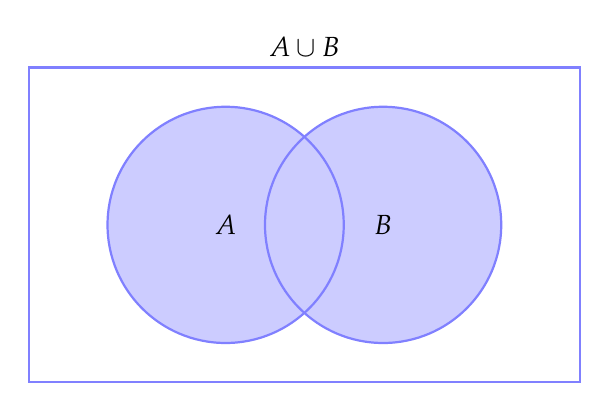
\begin{tikzpicture}
    \draw[outline] \firstrectangle;
    \draw[filled] \firstcircle node {$A$}
                  \secondcircle node {$B$};
    \node[anchor=south] at (current bounding box.north) {$A \cup B$};
\end{tikzpicture}
\end{center}
\columnbreak
\begin{description} 
 \item[L'intersection ({$\cap$}) :] On peut le voir comme un "et". Lorsqu'il est utilisé, on s'intéresse à savoir si un résultat est présent dans tous les ensembles impliqués.
\end{description}
\begin{itemize}
  	\item	Si l'événement $A$ est d'avoir un chiffre pair sur un dé et que l'événement $B$ est d'avoir 5 ou 6 sur ce même lancer de dé, le seul résultat possible de $A \cap B$ est 6, car 6 est un nombre pair et fait partie de l'ensemble $B$. 
  	\item Une notation alternative est de simplement écrire $AB$.
\end{itemize}
\begin{center}
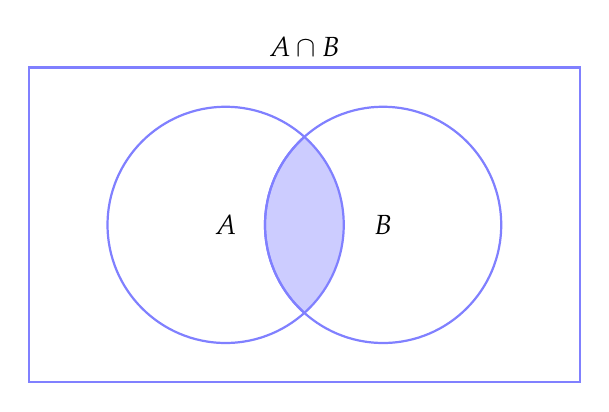
\begin{tikzpicture}
    \begin{scope}
        \clip \firstcircle;
        \fill[filled] \secondcircle;
    \end{scope}
    \draw[outline] \firstrectangle;
    \draw[outline] \firstcircle node {$A$};
    \draw[outline] \secondcircle node {$B$};
    \node[anchor=south] at (current bounding box.north) {$A \cap B$};
\end{tikzpicture}
\end{center}
\begin{description} 
 \item[Complémentaire :] Un événement $A^{c}$ est le complémentaire d'un événement A lorsqu'il correspond à tous les résultats de $\Omega$ excluant les résultats de $A$. 
\end{description}
\begin{itemize}
  	\item	Un exemple est l'événement "Avoir un nombre pair sur un dé"; un événement complémentaire serait donc "Avoir un nombre impair sur un dé".
  	\item   Le complémentaire d'un événement A est désigné par {$\overline{A}$}, $A^{c}$ et $A^{'}$.
\end{itemize}
\begin{center}
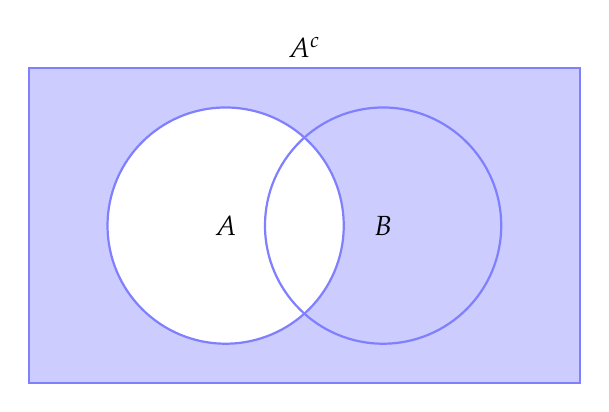
\begin{tikzpicture}
    \begin{scope}
    \fill [filled] \firstrectangle;
    \fill [white] \firstcircle;
    \end{scope}

    \draw[outline] \firstrectangle;
    \draw[outline] \firstcircle node {$A$};
    \draw[outline] \secondcircle node {$B$};
    \node[anchor=south] at (current bounding box.north) {$A^c$};
\end{tikzpicture}
\end{center}
\pagebreak
\begin{description} 
 \item[Inclusion ($\subset$) :] Afin de dire que l'événement B est compris dans l'événement A, on peut écrire le tout avec la notation suivante : $B \subset A$. On peut donc dire que tous les résultats de l'événement $B$ se retrouvent aussi dans l'événement $A$.
\end{description}
\begin{center}
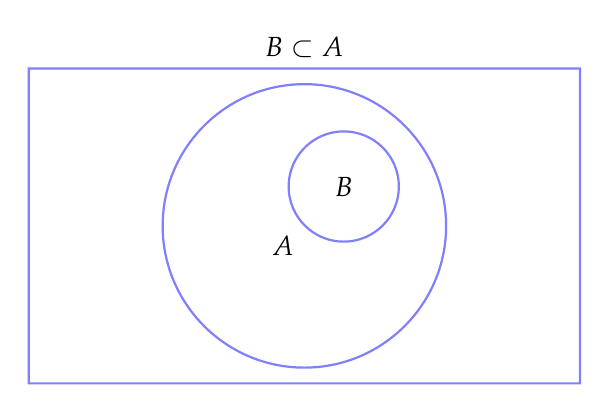
\begin{tikzpicture}
\draw[outline] \firstrectangle 
(3.5, 2) circle (1.8) node [text = black, below left]{$A$}
(4, 2.5) circle (0.7) node {$B$};
    \node[anchor=south] at (current bounding box.north) {$B \subset A$};
\end{tikzpicture}
\end{center}

\begin{definitionNOHFILL}[Événements mutuellement exclusifs]
Deux événements $A$ et $B$ sont dits mutuellement exclusifs lorsque l'intersection entre les deux événements est vide ($A \cap B = \emptyset$). C'est donc dire que $\Pr(A \cap B) = 0$.
\end{definitionNOHFILL}

\begin{definitionNOHFILLprop}[Propriétés des ensembles]
\begin{description}
  \item[Commutativité :] 
  $$A_1	\cup	A_2	=	A_2 \cup A_1$$ $$A_1	\cap	A_2	=	A_2 \cap A_1$$
  \item[Associativité :] $$(A_1 \cup A_2)	\cup A_3	=	A_1 \cup		(A_2 \cup A_3)$$ $$(A_1 \cap A_2)	\cap A_3	=	A_1 \cap		(A_2 \cap A_3)$$
  \item[Distributivité :] $$(A_1 \cup A_2)	\cap A_3 = (A_1 \cap A_3) \cup (A_2 \cap A_3)$$ $$(A_1 \cap A_2)	\cup A_3 = (A_1 \cup A_3) \cap (A_2 \cup A_3)$$
  \item[Loi de DeMorgan :] $$(\bigcup_{i = 1}^{n} A_{i})^{c} = (\bigcap_{i=1}^{n} A_i^{c})$$ $$(\bigcap_{i = 1}^{n} A_{i})^{c} = (\bigcup_{i=1}^{n} A_i^{c})$$
\end{description}
\end{definitionNOHFILLprop}
\vfill\null
\columnbreak

\subsection{Axiomes de probabilité}
\begin{definitionNOHFILLprop}[Axiomes de probabilité]
Supposons que pour chaque événement $E$ de $\Omega$ (espace échantillonnal d'une expérience aléatoire), il existe un nombre $\Pr(E)$. On peut appeler ce nombre $\Pr(E)$ la probabilité de E si celle-ci satisfait les axiomes ci-dessous. Autrement dit, ces axiomes sont des règles que les probabilités se doivent de respecter: 

\begin{description}
  \item[1)] $0 \leq \Pr(A) \leq 1$
  \item[2)] $\Pr(\Omega)=1$
  \item[3)] Si $A_i$ $\cap$ $A_j$ = $\emptyset$ pour $i \neq j$ (mutuellement exclusifs), alors $\Pr(\bigcup_{i = 1}^{n}$ $A_i) = \sum_{i = 1}^{n} \Pr(A_i)$
\end{description}
\end{definitionNOHFILLprop}

\begin{definitionNOHFILLprop}[Relations à savoir]

\begin{description}
  \item[1)] $\Pr(\emptyset) = 0$
  \item[2)] $\Pr(E^c) = 1 - \Pr(E)$
  \item[3)] Si $E \subset F$, alors $\Pr(E) \leq \Pr(F)$
  \item[4) (Formule de Poincaré)] \begin{align*} \Pr(E_1 \cup E_2 \cup ... \cup E_n) =& \sum_{i=1}^n \Pr(E_i) - \sum_{i_1<i_2} \Pr(E_{i_1} E_{i_2}) + ...+\\& (-1)^{r+1} \sum_{i_1<i_2<...<i_r} \Pr(E_{i_1}E_{i_2}...E_{i_r}) + ...+\\& (-1)^{n+1} \Pr(E_1E_2...E_n)
  \end{align*}
  \begin{itemize}
  \item À deux événements, on obtient :\\ $$\Pr(A \cup B) = \Pr(A) + \Pr(B) - \Pr(A \cap B)$$
  \item À trois événements, on obtient :\\
	\begin{align*}  
  \Pr(A \cup B \cup C) =& \Pr(A) + \Pr(B) + \Pr(C) - \\& \Pr(A \cap B) - \Pr(A \cap C) - \Pr(B \cap C) + \\& \Pr(	A \cap B \cap C)
  \end{align*}
  \end{itemize}
\end{description}
D'autres relations peuvent être déduites à l'aide d'un diagramme de Venn. Il faut toutefois utiliser la notation probabiliste à travers les calculs. Un diagramme de Venn avec de simples calculs \textbf{ne suffit pas} en examen.
\end{definitionNOHFILLprop}

\subsection{Résultats équiprobables}

\begin{definitionNOHFILL}[Résultats équiprobables]
Si chaque résultat de $\Omega$ a la même chance de se réaliser, on peut trouver la probabilité qu'un événement $A$ se réalise à l'aide de la formule suivante :\\ $$\Pr(A) = \frac{Nombre~de~r \acute{e} sultats~dans~A}{Nombre~de~r \acute{e} sultats~dans~\Omega}$$\\
Par exemple, si on cherche la probabilité d'obtenir un nombre pair au cours d'un lancer de dé, on peut utiliser la formule ci-dessus, car il y a autant de chances d'obtenir chacun des côtés d'un dé au cours d'un lancer. Ainsi, $\Pr$(Obtenir un nombre pair) $= \frac{3}{6} = \frac{1}{2}$
\end{definitionNOHFILL}
\vfill\null
\pagebreak

\section{Probabilité conditionnelle}

\subsection{Notation}
\begin{distributions}[Notation]
On utilise la notation suivante afin de désigner la probabilité que l'événement A se réalise sachant que l'événement B s'est réalisé : $\Pr(A|B)$.
\end{distributions}

\subsection{Relations à savoir}
\begin{definitionNOHFILLprop}[Relations à savoir]
\begin{description}
  \item[1)] On obtient tout d'abord :\\$$\Pr(A | B) = \frac{\Pr(A \cap B)}{\Pr(B)}.$$
  \item[2)] On peut calculer $\Pr(A \cap B)$ des deux façons suivantes :\\ $$\Pr(A \cap B) = \Pr(A | B)* \Pr(B)$$
  $$\Pr(A \cap B) = \Pr(B | A)* \Pr(A)$$\\On peut également généraliser ce résultat pour $n$ événements en utilisant la règle de multiplication:\\ $$\Pr(E_1 \cap E_2 \cap ... \cap E_n)= \Pr(E_1)* \Pr(E_2|E_1 \cap E_2)*... *\Pr(E_n|E_1 \cap E_2 ... \cap E_{n-1})$$\\
  \item[3)] On peut réécrire l'équation du point 1 de la façon suivante (à l'aide du point 2) : 
   $$\Pr(A | B) = \frac{\Pr(A \cap B)}{\Pr(B)} = \frac{Pr(B | A)* \Pr(A)}{\Pr(B)} $$ 
   \item[4) (Loi des probabilités totales)] $$\Pr(E) =	\sum_{i = 1}^{n} \Pr(E | F_{i}) \Pr(F_{i})$$
 Pour pouvoir appliquer cette relation, il faut que $F_i$ forment une partition de $\Omega$, c'est-à-dire que $\Pr(F_1) + \Pr(F_2) + ... + \Pr(F_n) = 1$ et qu'il n'y ait aucun résultat en commun pour aucune paire de $F_i$ (donc que $F_i \cap F_j = \emptyset $ pour toutes paires de $i$ et $j$).
\end{description}
\end{definitionNOHFILLprop}

\begin{definitionNOHFILLprop}[Relations à savoir (suite)]
\begin{description}

  \item[5) (Théorème de Bayes)] 
  Si on reprend la formule du point 3, et qu'on applique la loi des probabilités totales au dénominateur, on obtient la formule de Bayes.
  
  \begin{align*}
  \Pr(A | B) &= \frac{\Pr(A \cap B)}{\Pr(B)} \\&= \frac{Pr(B | A)* \Pr(A)}{\Pr(B)} \\&= \frac{Pr(B | A)* \Pr(A)}{Pr(B | A)* \Pr(A) + \Pr(B|A^c) *  \Pr(A^c)}
  \end{align*} \\

  On peut également généraliser ce résultat pour un ensemble d'événements $\{F_1,F_2,...,F_n\}$ qui forment une partition de $\Omega$.
  
  $$ \Pr(F_j | E) = \frac{\Pr(E | F_{j}) \Pr(F_{j})}{\sum_{i = 1}^{n} \Pr(E | F_{i}) \Pr(F_{i})} $$
\end{description}
\begin{distributions}[Indépendance]
S'il y a indépendance entre les événements ($A$ n'a aucun impact sur $B$, et vice-versa), les relations suivantes sont vraies:\\
$$\Pr(A|B) = \Pr(A)$$
$$\Pr(A \cap B) = \Pr(A)*\Pr(B)$$\\
On peut également généraliser ces relations lorsqu'il y a plusieurs événements mutuellement indépendants.\\
\\ Assurez-vous de bien distinguer les événements indépendants des événements mutuellement exclusifs ($\Pr(A \cap B) = 0$ pour les événements mutuellement exclusifs).
\end{distributions}
\end{definitionNOHFILLprop}

\begin{formula}{Démarche afin de répondre aux questions contextuelles du chapitre 2 et 3}
Concernant les questions contextuelles (donc avec une mise en situation) portant sur les notions du chapitre 2 et chapitre 3, voici une démarche qui devrait vous aider.
\\

\textbf{Exemple} : il y a deux types d'assurés. Il y a les bons assurés et les mauvais assurés. La probabilité qu'un bon assuré ait au moins $1$ accident cette année est de $20~\%$. La probabilité qu'un mauvais assuré n'ait pas d'accident cette année est de $70~\%$. Également, il y a 3 fois plus de bons assurés que de mauvais assurés. \textbf{Quelle est la probabilité que, sachant qu'un assuré a eu au moins un accident au cours de l'année, celui-ci soit un mauvais assuré?}\\

\begin{description}
\item [1)] \textbf{Il faut bien définir les événements.}\\

$A :$ L'assuré est un bon assuré.\\
$B :$ L'assuré a au moins 1 accident au cours de l'année.\\

\item [2)]\textbf{Il faut bien définir les informations présentes dans le texte sous notation probabiliste. La notation doit être cohérente avec la définition des événements.}
$$\Pr(A) = 3\Pr(A^c)$$ $$\Pr(B|A) = 0.2$$ $$\Pr(B^c|A^c) = 0.7$$ \item [3)] \textbf{Il faut bien définir l'information recherchée sous notation probabiliste. Encore une fois cette notation doit être cohérente avec la définition des événements.} \\

On cherche $\Pr(A^c|B)$.\\
\item [4)] \textbf{Selon les informations données, on applique une ou plusieurs des relations présentées dans le chapitre 2 ou dans le chapitre 3. Cette partie est la plus difficile, et c'est à force de faire des numéros qu'on reconnait quelles relations utiliser.}\\

Dans ce cas-ci, on peut développer la probabilité recherchée de la façon suivante :\\
$$\Pr(A^c | B) = \frac{\Pr(A^c \cap B)}{\Pr(B)}.$$\\
Puisqu'on n'a aucune information sur $\Pr(A^c \cap B)$ et sur $\Pr(B)$, on développe cette formule davantage (on obtient le théorème de Bayes) :\\$$\frac{\Pr(A^c \cap B)}{\Pr(B)} = \frac{Pr(B | A^c)* \Pr(A^c)}{Pr(B | A)* \Pr(A) + \Pr(B|A^c) *  \Pr(A^c)}.$$\\
Ici, on peut trouver $\Pr(A)$, $\Pr(A^c)$ et $\Pr(B|A^c)$ à l'aide de la relation qui relie les probabilités d'événements complémentaires et des informations données dans l'exemple.\\
$$\Pr(A) = 1 - \Pr(A^c)$$
$$ 3 \Pr(A^c) = 1 - \Pr(A^c)$$
$$ \Pr(A^c) = \frac{1}{4}$$\\
Et donc, $\Pr(A^c) = \frac{1}{4}$ et $\Pr(A) = \frac{3}{4}$. Pour trouver $\Pr(B|A^c)$ :\\
$$\Pr(B|A^c) =  1 - \Pr(B^c|A^c) = 0.3.$$\\ En remplaçant ces valeurs dans la formule de Bayes (et en utilisant $\Pr(B|A) = 0.2$, soit une information qui nous était déjà fournie), on obtient $$\Pr(A^c|B) = \frac{1}{3}. $$
\end{description}
\end{formula}


\subsection{Montrer l'indépendance}
\begin{definitionNOHFILL}[Montrer l'indépendance]
Si on veut montrer que deux événements  ($A$ et $B$) sont indépendants, on veut montrer la relation suivante : \\
$$ \Pr(A \cap B) = \Pr(A) * \Pr(B) $$\\
On veut montrer que les deux côtés de l'égalité sont égaux. Faites attention à la façon dont vous calculez $\Pr(A \cap B)$. Il ne faut pas calculer ce terme en faisant $\Pr(A) * \Pr(B)$. Il faut absolument dénombrer les résultats se situant dans $A \cap B$.\\
\\
Si on veut montrer que trois événements ($A$, $B$ et $C$) sont mutuellement indépendants, on veut montrer les quatre relations suivantes : \\
$$\Pr(A \cap B) =  \Pr(A) * \Pr(B)$$
$$\Pr(A \cap C) =  \Pr(A) * \Pr(C)$$
$$\Pr(B \cap C) =  \Pr(B) * \Pr(C)$$
$$\Pr(A \cap B \cap C) =  \Pr(A) * \Pr(B) * \Pr(C).$$
\end{definitionNOHFILL}
\vfill\null
\pagebreak

   
   



\pagebreak
\section{Chapitre 4:\\ Variable aléatoire discrète}
\begin{probch4}{La variable aléatoire}
  \begin{description}
    \item[Définition :] Nous avons déjà vu que les événements sont délimités par l'ensemble échantillonnal S, c'est-à-dire les résultats possibles de l'événement. La variable aléatoire, disons X, sera une fonction de cet ensemble S (S $\in$ $\mathbb{R}$).\\
    Le support, que l'on peut comparer à l'image de la fonction, d'un événement X est composé des résultats possibles d'une expérience, par exemple [0, 1] ou encore un ensemble dénombrable comme \{0, 1/2, 1\}.\\
    Pour bien comprendre la différence entre l'espace échantillonnal et le support de X, voici un petit exemple : \\
    On lance une pièce de monnaie deux fois et on définit la variable aléatoire X comme étant le nombre de faces obtenus. L'espace échantillonnal de l'expérience est \{(P,P), (P,F), (F,P), (F,F)\} et le support de X est de \{0, 1, 2\}.
	\item [Fonction de masse de probabilité :] La probabilité d'avoir un résultat égal à x. Cette fonction est définie par $\Pr(X = x_i)$ 
	\item[Fonction de répartition ($F_{X} (x)$):] La probabilité d'avoir un résultat inférieur à x.
    \begin{align*}
    F_{X} (x) &= \Pr(X \le x) \\
    &= \sum_{x_{i} \le x}^{} \Pr(X = x_{i})
    \end{align*}
    Pour illustrer la fonction de répartition, on peut s'imaginer un lancer de dé et définir X comme le résultat du lancer. $F_{X} (2)$, par exemple, donnerait alors 1/3 car seuls les résultats 1 et 2 sont considérés sur l'ensemble des 6 possibilités. 
    \item[Propriétés de la fonction de répartition :] La valeur de la fonction de répartition se situe toujours entre 0 et 1, ce qui est logique étant donné que la somme de toutes les probabilités est toujours égale à 1 et qu'il n'existe pas de probabilité inférieure à 0. \\
    La fonction est aussi toujours non-décroissante, car il est impossible de perdre des probabilités alors que les probabilités qui s'ajoutent à mesure que x augmente sont toujours supérieures à 0 (pour une variable aléatoire discrète, cela donne une fonction en escalier à droite).\\
    On sait donc que $F_{X} (a) \le F_{X} (b)$ pour a < b. On peut alors trouver que Pr(a < X $\le$ b) = $F_{X} (b) - F_{X} (a)$.
    \item[Fonction de répartition inverse ($F^{-1}_{X} (u)$):] Aussi nommée la fonction quantile, cette fonction sert à déterminer quel résultat correspond à une quantité u de probabilités accumulées. Par exemple, si je prends un u de 0,5, le résultat sera la médiane. \\
	Cela fonctionne de la façon suivante : on remplace le x de la fonction de répartition par u et cette nouvelle fonction est mise égale à x et on isole le u. Autrement dit, il faut trouver une fonction réciproque. \\
	\item[Espérance :] L'espérance correspond à une moyenne pondéré des probabilités où les pondérations correspondent aux différents valeurs que peut prendre la variable $X$. Elle est définie de la façon suivante: \\
	$$ E[X] = \sum_i x_i * \Pr(X = x_i) $$. L'espérance correspond au résultat espéré lors de l'expérience. Par exemple, l'espérance d'une expérience consistant à lancer un dé serait 3.5. De plus, \\
	il est possible de calculer l'espérance d'une fonction $g(X)$. L'espérance, dans ce cas-ci, est définie de la façon suivante : $E[g(X)] = \sum_i g(x_i) * \Pr(X = x_i) $. \\
	\item[Propriétés de l'espérance: ] L'espérance est un opérateur linéaire. Ainsi, $E[2x^2+6x+5]$ peut se réécrire, une fois simplifiée, $2E[X^2]+6E[X]+5$. Aussi, si $g(x) \le h(x)$, $\forall x$, alors $E[g(x)] \le E[h(h)]$. \\
	\item[Variance :] La variance est une mesure de dispersion qui se trouve à être la moyenne du carrée des écarts entre x et sa moyenne. La variance est définie de la façon suivante : $ Var(X) = E[(X - E[X])^2]$. En développant cette \\ 
	expression, on retrouve l'expression davantage utilisée en probabilité, soit $Var(X) = E[X^2] - (E[X])^2$.  Afin de calculer la variance on trouve habituellement le premier et le deuxième moment de X et on remplace dans la formule. \\
	De plus, la variance n'est pas un opérateur linéaire. Cependant, $Var(aX + b) = a^2 Var(X)$ où $a$ et $b$ sont des constantes réelles.
\end{description}
\end{probch4}
\end{multicols*}

\end{document}
